% 第4章
%!TEX root = main.tex

%%%%%%%%%%%%%%%%%%%%%%%%
\chapter{パラメータ同定}
\label{sys_id}
%%%%%%%%%%%%%%%%%%%%%%%%

本章では,開発機体を用いた実験で得た飛行データをもとに,モデル内の未知パラメータを同定する手順および手法について述べる.高次元モデルを用いて正確なパラメータ推定を行なうことは困難であるため,ここまでに記述した低次元モデル,中でも縦運動にのみ注目しさらに低次元化したモデルを用いて推定を行なう.ただし,縦運動と横運動に分ける際に,それぞれの干渉を無視した条件を与えることになる.そのため,単純に低次元化しただけでは欲しい実験データ取得の困難性が残る.そこで,プロの操縦者に協力してもらい,できる限り各運動に限定したデータ取得を行なっている.\label{da}

%%%%%%%%%%%%%%%%%%%%%%%%
\section{データの前処理}
%%%%%%%%%%%%%%%%%%%%%%%%

本節では,IMUから取得した飛行ログデータの前処理について述べる.前処理としては,そのまま扱うことができないものについての補正と,データのフィルタリングに大きく分けられる.

\subsection{センサ取り付け位置の補正}

各運動モデルは機体座標系の原点を基準として構成されているが,原点位置にセンサを取り付けることができない構造であるため,その分の補正が必要である.ここでは,取り付け位置によって変化する速度の補正について述べる.Fig. \ref{fig:location_IMU},~\ref{fig:IMU_position}に示すように,加速度センサは機体軸原点からベクトル$\mbox{\boldmath $R_{p2B}$}$だけ離れた位置に取り付けられている.このとき,機体軸原点の速度は
\begin{equation}
  \mbox{\boldmath $V$} = \dfrac{d}{dt}\mbox{\boldmath $R_B$} = \dfrac{d}{dt}(\mbox{\boldmath $R_p$}+\mbox{\boldmath $R_{p2B}$})\triangleq \mbox{\boldmath $\dot{R}_p$}+\mbox{\boldmath $\dot{R}_{p2B}$}
\end{equation}
で与えられる.したがって,$\mbox{\boldmath $\dot{R}_{p2B}$}$によってセンサ位置によるずれを補正する.このベクトルの機体座標表現は
\begin{equation}
  \mbox{\boldmath $\dot{R}_{p2B}$} = \mbox{\boldmath $\omega_p$}\times\mbox{\boldmath $R_{p2B}$} =
  \left[
    \begin{array}{ccc}
      p \\
      q \\
      r
    \end{array}
  \right] \times
  \left[
    \begin{array}{ccc}
      -l_{px} \\
      0 \\
      l_{pz}
    \end{array}
  \right] =
  \left[
    \begin{array}{ccc}
      ql_{pz} \\
      -rl_{px} + pl_{pz} \\
      ql_{px}
    \end{array}
  \right]
\end{equation}
と計算できる.

\begin{figure}[htbp]
	\begin{center}
		\begin{tabular}{c}
			\begin{minipage}{0.5\hsize}
				\begin{center}
					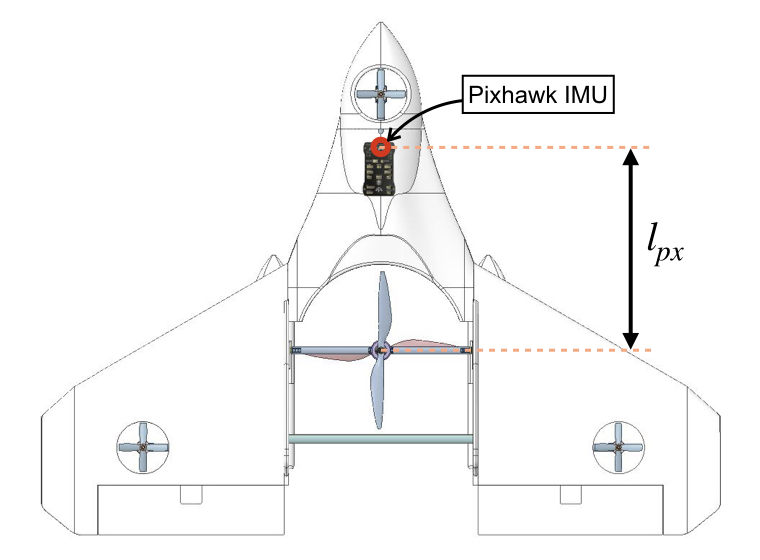
\includegraphics[clip,width=7.0cm,bb=0 0 800 600]{./z_figure_files/chapter4/1_location_IMU.jpeg}
					\caption{Location of acceleration sensor}
					\label{fig:location_IMU}
				\end{center}
			\end{minipage}
			\begin{minipage}{0.5\hsize}
				\begin{center}
					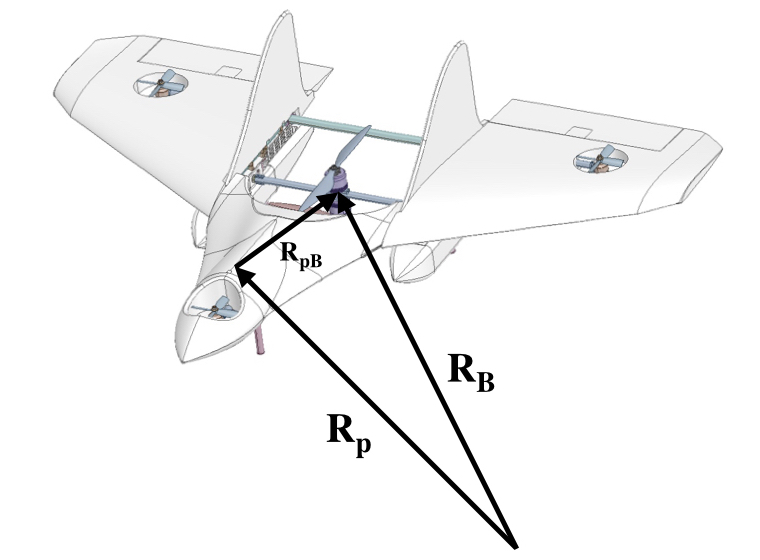
\includegraphics[clip,width=7.0cm,bb=0 0 800 600]{./z_figure_files/chapter4/2_IMU_position.jpeg}
					\caption{Consideration of sensor position}
					\label{fig:IMU_position}
				\end{center}
			\end{minipage}
		\end{tabular}
	\end{center}
\end{figure}

\subsection{風の影響の補正}

実験は,屋外で風外乱の環境下にて,回転翼機モードにおいて行なった.対気速度の測定のために,機首先端にピトー管が取り付けられているが,回転翼機モードでの飛行時は測定誤差が大きいことが分かっている.そこで,風速計を機体の進行方向と同じ向きに設置し,風速を測定した.データ処理時には,風速計による計測ログと機体の対地速度,および機体姿勢ログを用いて,\ref{sec:wind_speed}小節の通り対気速度を計算する.

\subsection{機体の加速度の算出}

計算に必要な機体の加速度$\mbox{\boldmath $\dot{V_g}$}$,角加速度$\mbox{\boldmath $\dot{\omega}$}$,および迎角速度$\dot{\alpha}$は,ログデータからも直接得られるが,誤差が大きいため計算により求める.機体の速度$\mbox{\boldmath $V_g$}$,角速度$\mbox{\boldmath $\omega$}$,および迎角$\alpha$はログデータから得られるため,これらの差分から計算する.時間遅れを考慮し中心差分法を用いて,加速度を代表して$\dot{u}$について表記すると
\begin{equation}
  \dot{u}_{[k]} = \dfrac{u_{[k+1]}-u_{[k-1]}}{2\Delta t}
\end{equation}
のように計算できる.$\Delta t$はログデータのサンプリング間隔であり,$k=1,2,3\hdots,n$はログデータのステップ数を表す.ただし,計算することができない左右境界の値は,ログデータから直接取得した値を採用する.

\subsection{各ロータ出力の評価}

メインロータおよびサブロータは,ログデータから得られる指令値(PWM値)を変換することによって推力値を得られる.この変換は,実験室内での予備実験により得られた測定結果から,計算結果と実際の推力との差が小さくなるように工夫して概算している.\cite{}

\subsection{データのフィルタリング}
\label{sec:filter}

センサで取得したログデータには,ノイズが含まれているためそのままでは使えず,必要な信号成分を取り出す必要がある.そこで,後に\ref{sec:analyze}節で述べる解析結果から,おおよその機体の固有振動数を算出し,入力や制御の周波数も考慮して,ログデータに対して$10\mathrm{[Hz]}$をカットオフ周波数としたローパスフィルタをかけた.サンプリング間隔は$0.02\mathrm{[s]}$であるから,サンプリング周波数は$50\mathrm{[Hz]}$である.フィルタの実現には高速フーリエ変換を用いた.フィルタ前後でどれだけノイズが除去されているかは,ある実験データのピッチ角速度を例に,Fig. \ref{fig:f_filter}に示す.

\begin{figure}[H]
	\centering
	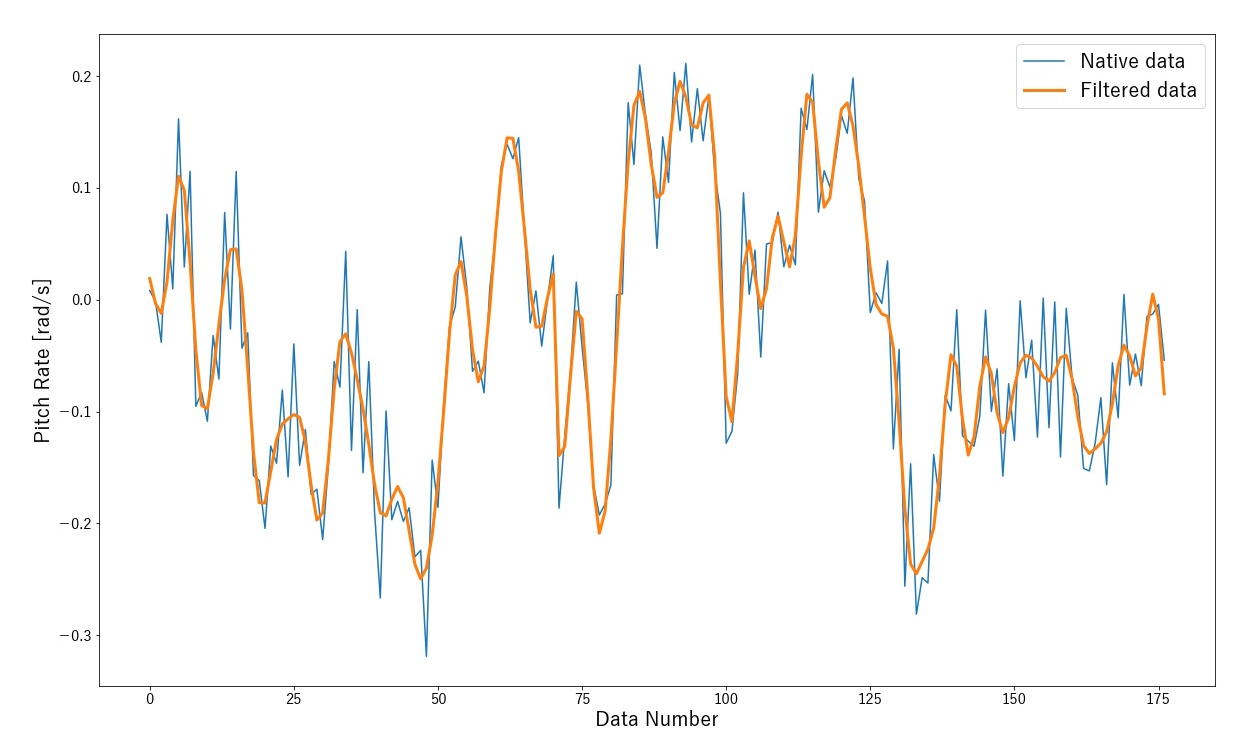
\includegraphics[clip,width=13.0cm,bb=0 0 1250 750]{./z_figure_files/chapter4/3_filter.jpeg}
	\caption{Filter pitch rate}
	\label{fig:f_filter}
\end{figure}

% 補正が必要なデータとして,次の項目が挙げられる.
% \begin{itemize}
% \item[(1)]センサ取り付け位置の補正
% \item[(2)]風の影響の補正
% \item[(3)]各ロータ出力の評価
% \item[(4)]気温や気圧による気体密度変化の考慮
% \end{itemize}



%%%%%%%%%%%%%%%%%%%%%%%%%%%%%%
\section{パラメータの推定手法}
%%%%%%%%%%%%%%%%%%%%%%%%%%%%%%

まず,モデル内の未知パラメータについて述べる.\ref{sec:lng_non_linear}小節に示したモデルにおいて,空気力項に未知パラメータが含まれる.ただし,\ref{sec:airspeed_airf}小節の空気力モデル式については,計算の際に式を変形して
\begin{equation}
  \left\{
  \begin{align}
    L &= \dfrac{1}{2}\rho {V_a}^2 S C_L^{\prime}, \quad C_L^{\prime} = \dfrac{L}{\frac{1}{2}\rho {V_a}^2 S} \\[5pt]
    D &= \dfrac{1}{2}\rho {V_a}^2 S C_D^{\prime}, \quad C_D^{\prime} = \dfrac{D}{\frac{1}{2}\rho {V_a}^2 S} \\[5pt]
    M_a &= \dfrac{1}{2}\rho {V_a}^2 S \bar{c} C_m^{\prime}, \quad C_m^{\prime} = \dfrac{Ma}{\frac{1}{2}\rho {V_a}^2 S \bar{c}}
  \end{align}
  \right
  \label{eq:L_D_Ma}
\end{equation}

\begin{equation}
  \left\{
  \begin{align}
    C_L^{\prime} &= C_{L_0}+C_{L_\alpha}\alpha+C_{L_{\dot{\alpha}}}\dfrac{\bar{c}}{2V_a}\dot{\alpha}+C_{L_q}\dfrac{\bar{c}}{2V_a}q+C_{L_{\delta_e}}\delta_e+\uwave{C_{L_k}\dfrac{1}{V_a}} \\[5pt]
    C_D^{\prime} &= C_{D_0}+\kappa C_L^2+\uwave{C_{D_k}\dfrac{1}{V_a}} \\[5pt]
    C_m^{\prime} &= C_{m_0}+C_{m_\alpha}\alpha+C_{m_{\dot{\alpha}}}\dfrac{\bar{c}}{2V_a}\dot{\alpha}+C_{m_q}\dfrac{\bar{c}}{2V_a}q+C_{m_{\delta_e}}\delta_e+\uwave{C_{m_k}\dfrac{1}{V_a}}
  \end{align}
  \right
  \label{eq:CL_CD_Cm}
\end{equation}
とする.以上より推定対象となるパラメータ$\xi$は
\begin{equation}
  \xi = [
  C_{L_0},
  C_{L_\alpha},
  C_{L_\dot{\alpha}}},
  C_{L_q},
  C_{L_{\delta_e}},
  C_{L_k},
  C_{D_0},
  \kappa,
  C_{D_k},
  C_{m_0},
  C_{m_\alpha},
  C_{m_\dot{\alpha}}},
  C_{m_q},
  C_{m_{\delta_e}},
  C_{m_k}
  ]
\end{equation}
となり,合計15個である.$\xi$に含まれていない変数は,実機実験からログデータとして直接取得可能か,あるいは計算が可能なものであり,パラメータ推定はすべてオフライン処理となる.\ref{sec:lng_non_linear}小節のモデル式より,$X_a,Z_a,M_a$はそれぞれ計算で求められ,式(\ref{eq:XZ_to_LD})より
\begin{equation}
  \left[
  \begin{array}{ccc}
    L \\
    D
  \end{array}
  \right] =
  \left[
  \begin{array}{ccc}
    \sin\alpha & -\cos\alpha \\
    -\cos\alpha & -\sin\alpha
  \end{array}
  \right]
  \left[
  \begin{array}{ccc}
    X_a \\
    Z_a
  \end{array}
  \right]
  \label{eq:LD_to_XZ}
\end{equation}
とかけて,$L,D$も計算で求められる.このようにログデータから算出した$L,D,M_a$は,添字を付けて$L_{log},D_{log},M_{a_{log}}$と表すことにする.

\hspace{5pt}

次に,推定手法について述べる.推定には最小二乗法を用いる.例えば,式(\ref{eq:CL_CD_Cm})を用いた揚力係数$C_L$についての最小二乗問題は,次のように策定される.
\begin{equation}
  \mbox{\boldmath $z$} = \mbox{\boldmath $X$}\mbox{\boldmath $\theta$} + \mbox{\boldmath $\nu$}
\end{equation}
となる.ここで,
\begin{equation*}
  \mbox{\boldmath $z$} =
  \left[
  \begin{array}{c}
    C_L^{\prime}(1) \quad C_L^{\prime}(2) \quad \hdots \quad C_L^{\prime}(N)
  \end{array}
  \right]^{\mathrm{T}} :
  \mbox{式(\ref{eq:L_D_Ma})から計算される$N\times1$ベクトル}
\end{equation*}
\begin{equation*}
  \mbox{\boldmath $\theta$} =
  \left[
  \begin{array}{c}
    C_{L_0} \quad C_{L_\alpha} \quad C_{L_\dot{\alpha}}} \quad C_{L_q} \quad C_{L_{\delta_e}} \quad C_{L_k}
  \end{array}
  \right]^{\mathrm{T}} :
  \mbox{未知パラメータの$6\times1$ベクトル}
\end{equation*}
\begin{equation*}
  \mbox{\boldmath $X$} =
  \left[
  \begin{array}{c}
    \mbox{\boldmath $1$} \quad
    \mbox{\boldmath $\alpha$} \quad
    \dfrac{\bar{c}}{2 \mbox{\boldmath $V_a$}} \mbox{\boldmath $\dot{\alpha}$} \quad
    \dfrac{\bar{c}}{2 \mbox{\boldmath $V_a$}} \mbox{\boldmath $q$} \quad
    \mbox{\boldmath $\delta_e$} \quad
    \dfrac{1}{\mbox{\boldmath $V_a$}}
  \end{array}
  \right] :
  \mbox{ログデータから得られる$N\times6$行列}
\end{equation*}
\begin{equation*}
  \mbox{\boldmath $\nu$} =
  \left[
  \begin{array}{c}
    \nu(1) \quad \nu(2) \quad \hdots \quad \nu(N)
  \end{array}
  \right]^{\mathrm{T}} :
  \mbox{誤差の$N\times1$ベクトル}
\end{equation*}

\hspace{5pt}

このとき推定したい$\mbox{\boldmath $\theta$}$は,モデルから想定される理論値と実際の測定値との差の二乗和である
\begin{equation}
  \mbox{\boldmath $J(\theta)$} = \dfrac{1}{2}(\mbox{\boldmath $z$}-\mbox{\boldmath $X\theta$})^{T}(\mbox{\boldmath $z$}-\mbox{\boldmath $X\theta$})
\end{equation}
を最小にするように定めればよい.したがって,最小二乗法\cite{}により推定値は
\begin{equation}
  \mbox{\boldmath $\hat{\theta}$} = (\mbox{\boldmath $X$}^{T}\mbox{\boldmath $X$})^{-1}\mbox{\boldmath $X$}^{T}\mbox{\boldmath $z$}
\end{equation}
と計算できる.

同様の手順で,抗力係数$C_D$とピッチモーメント係数$C_m$についても計算すれば,未知パラメータ群$\xi$はすべて求めることができる.実際の推定結果とそれに対する考察は,\ref{sec:}節で行なう.
